\documentclass[10pt]{article}
\usepackage{geometry}
\usepackage{graphicx}
\usepackage{wrapfig}
\usepackage{parskip}
\geometry{left=1.5cm,right=1.5cm,top=1.5cm,bottom=2cm}
\usepackage{gensymb}
\usepackage{caption}
\usepackage{xcolor}
\usepackage{amsmath}
\usepackage{float}  
\usepackage{subfigure}



\begin{document} 

\title{\huge{COMP6245(20/21): Foundations of Machine Learning (MSc) Lab 1 Report}}
\author{\normalsize{Yan Zhang (yz10u20@soton.ac.uk)}}
\date{}
\maketitle


\section{Introduction}

The Gaussian distribution(also known as Normal distribution) is widely used in the area of machine learning. In this report, I use mathematical methods to give answer to the tasks listed in the Lab 1 pages. 

\section{Solution}
\subsection{Preliminaries}
In the Preliminaries, the 3 by 3 symmetric matrix B is created. We found that the dot product of the first two column of the eigenvectors matrix is close to 0. We assume that the product of the eigenvectors of a symmetric matrix is orthogonal. 

Let $v_{1}$, $v_{2}$ be eigenvectors of matrix B corresponding to the eigenvalues $\alpha$,$\beta$, 
we have
\begin{equation}
   Bv_{1} = {\alpha}v_{1}, Bv_{2} = {\beta}v_{2}
\end{equation}
To prove that u and v are orthogonal, we can conclude this by showing the inner product $v_{1}v_{2}=0$. Then compute
\begin{equation}
\begin{aligned}
{\alpha}(v_{1}v_{2}) = ({\alpha}v_{1})v_{2}
  = Bv_{1}v_{2} = (Bv_{1})^{T}v_{2}\\
  = v_{1}^{T}B^{T}v_{2} = v_{1}^{T}Bv_{2}
  = v_{1}^{T}{\beta}v_{2} = {\beta}(v_{1}^{T}v_{2})
  = {\beta}(v_{1}v_{2})
\end{aligned}
\end{equation}
we have 
\begin{equation}
\begin{aligned}
    {\alpha}(v_{1}v_{2}) = {\beta}(v_{1}v_{2})\\
    ({\alpha}-{\beta})v_{1}v_{2} = 0
\end{aligned}
\end{equation}
Because ${\alpha}-{\beta}\neq0$. Hence, we must have $v_{1}v_{2}=0$ and the eigenvectors are orthogonal. We now come to the conclusion that eigenvectors of real symmetric matrices are orthogonal. 

\subsection{Random Numbers and Uni-variate Densities}

Now we consider generate sample from continuous uniform distribution. we randomly generated two groups of 1000 sample from the U(0,1) distribution, one with the bins = 4 and another with the bins=40. The figure of the histogram is shown in figure 1.

\begin{wrapfigure}{r}{0.7\textwidth}
\vspace{-7mm}
\hspace{20mm}
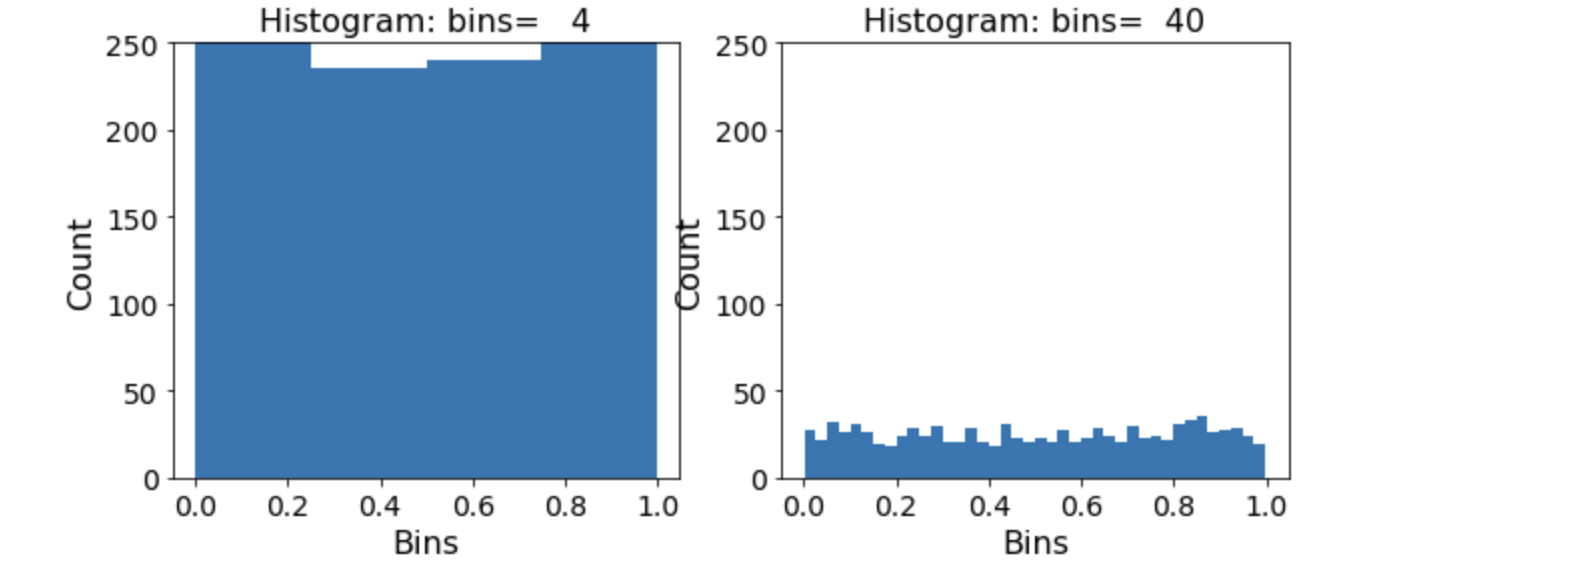
\includegraphics[width=0.7\linewidth]{1000samples.png} 
\caption{\footnotesize The two histograms showing the count of samples in each bin with bins=4 and bins=40.}
\end{wrapfigure}

The data is from a uniform distribution, where the probability of generating each data is equal. However, the figure does not appear flat, and there are some small ups and downs in the hist. This is because when sampling data from the uniform distribution, the sampling error exists. A sampling error is a statistical error that occurs when a sample is selected that does not represent the whole population. In this case, the sampling error is only an approximation of the population from which it is drawn, which means a certain range of bin could probably contain more data, and vice versa. After many repeated experiments, the plotted graph looks slightly different. Many reason could contribute to this result. Concretely, every time a sample is selected, there is a probability of being selected and a probability of not being selected. Hence, In every experiment, there might be some difference in the samples that were selected.

\begin{wrapfigure}{r}{0.7\textwidth}
\centering 
\vspace{-7mm}
\hspace{20mm}
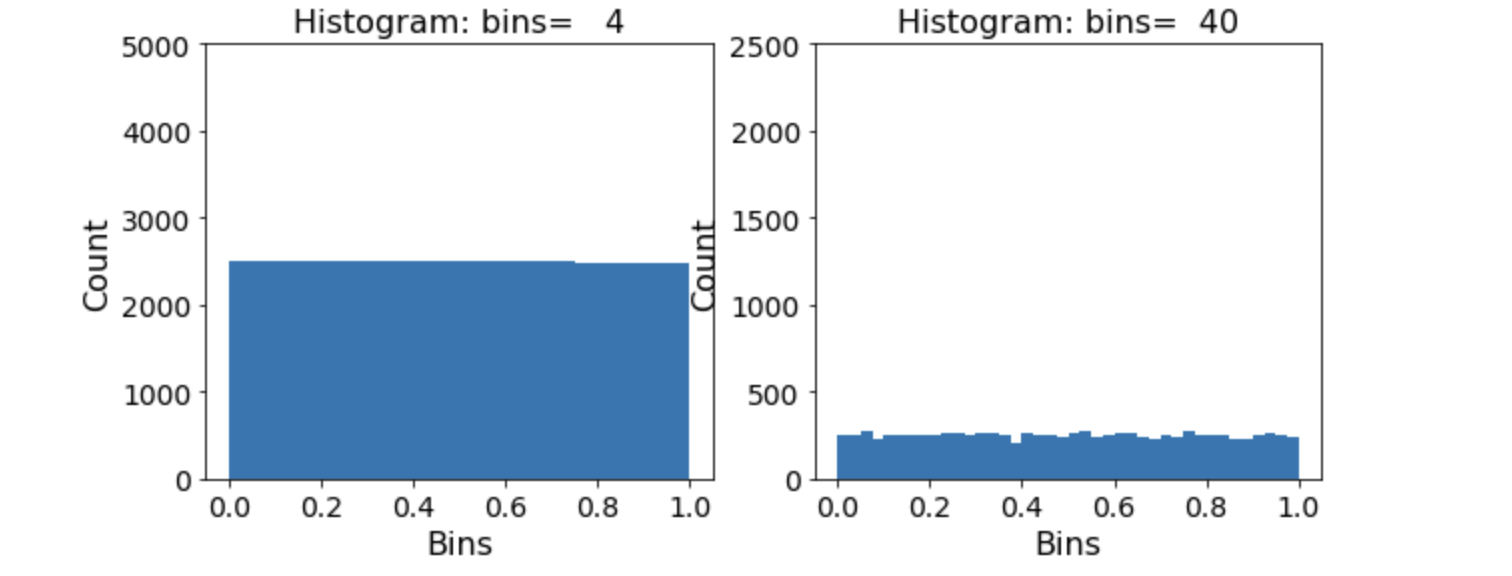
\includegraphics[width=0.7\linewidth]{10000samples.png} 
\caption{\footnotesize The two histograms showing the count of samples in each bin with bins=4 and bins=40.}
\centering
\end{wrapfigure}

When starting with more data(10000 samples), the histogram appears flat. The smaller the sampling error is, the histogram appears flatter. In this case, when we start with a larger sample size, the sampling error is almost eliminated and most of the data points represent the whole population which overwhelm the disorder caused by a small part of the data points. Although it is good to have low sampling error, but large sampling size requires more resource and time.

\begin{wrapfigure}{r}{0.7\textwidth}
\centering 
\vspace{-7mm}
\hspace{20mm}
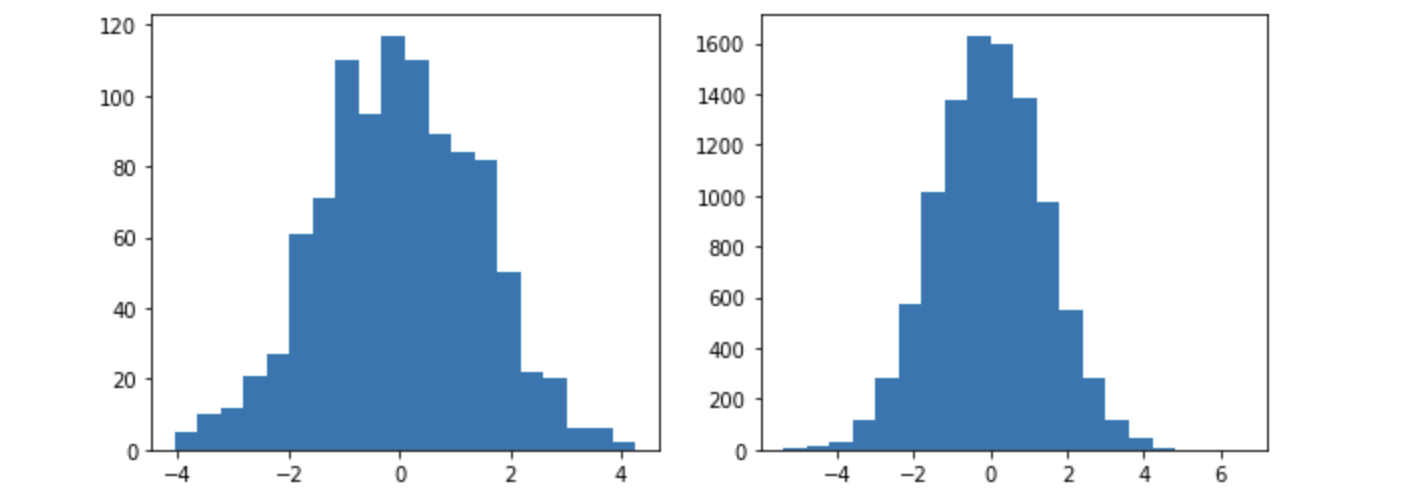
\includegraphics[width=0.7\linewidth]{sumofuniform2.png} 
\caption{\footnotesize  Distribution of the subtract of sum of uniform random distribution of size 1000 and 10000}
\centering
\end{wrapfigure}

Now, we add some uniform random numbers of size 1000, subtract the sum of each of them, and plot the histogram. The histogram looks like it is shaped like a curve approximate to normal distribution(shown in the first graph in Figure 3). The second graph in figure3 shows the histogram that when we started with more data. It appears that when the sample size goes up, the width of curve is getting gradually smaller. Hence larger sample gave us a more accurate estimate of the population mean. According to the central limit theorem, the mean of a sufficiently large number of independent random variables will itself be approximately normally distributed. In our case, the subtract of sum of samples is equal to the mean of the samples, because they both represent the center the whole samples. 

\subsection{Uncertainty in Estimation}

\begin{wrapfigure}{r}{0.7\textwidth}
\centering 
\vspace{-5mm}
\hspace{20mm}
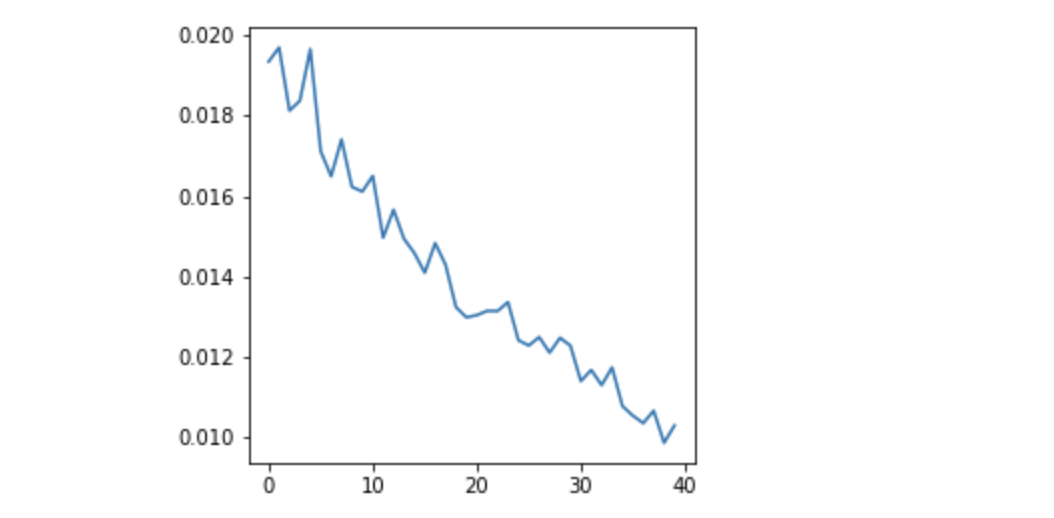
\includegraphics[width=0.5\linewidth]{UncertaintyInEstimation.png} 
\caption{\footnotesize  The variance of a uni-variate Gaussian density}
\centering
\end{wrapfigure}

There are many uncertainties in estimating the parameters in machine learning model. we want to estimate the variance of a uni-variate Gaussian, and the Figure 4 shows that as the sample size go up, the variation will be small. The sample size dictates the amount of information we have, and determine the precision that our estimation has. The uncertainty in our estimation is also determined by in confidence interval we made.

For a known standard deviation, the confidence interval is the form:
\begin{equation}
    \centering
     \big( \overline{x}-z^*\frac{\sigma }{\sqrt{n} } ,\overline{x}+z^*\frac{\sigma }{\sqrt{n} }\big) 
    \centering
\end{equation}
where $z^*$= $\Phi^{-1} \big(1- \frac{\alpha}{2} \big)=- \Phi^{-1}\big(\frac{\alpha}{2}\big)$

As the sample size $n$ increases, confidence interval gets larger so the uncertainty in the estimation decreases. 

%\newpage
\subsection{Bi-variate Gaussian Distribution}

The Bi-variate Gaussian distribution is clearly visualized by the 3 dimension contour plot, which is shown in Figure 5.

\begin{figure} %这里使用的是强制位置,除非真的放不下,不然就是写在哪里图就放在哪里,不会乱动
	\centering  %图片全局居中
	\vspace{-0.35cm} %设置与上面正文的距离
	\subfigtopskip=2pt %设置子图与上面正文或别的内容的距离
	\subfigbottomskip=2pt %设置第二行子图与第一行子图的距离,即下面的头与上面的脚的距离
	\subfigcapskip=-5pt %设置子图与子标题之间的距离
	\subfigure[$\mu = \begin{bmatrix}0 ,& 2\end{bmatrix} \sigma= \begin{bmatrix}2 & 1 \\1 & 2 \end{bmatrix} $]{
		\label{level.sub.1}
		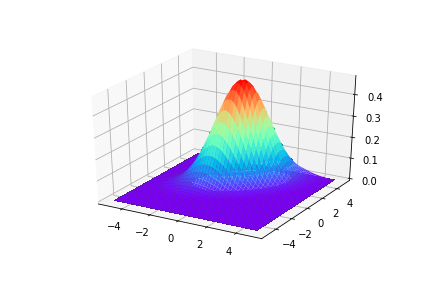
\includegraphics[width=0.32\linewidth]{contour1.png}}
	\quad %默认情况下两个子图之间空的较少,使用这个命令加大宽度
	\subfigure[$\mu = \begin{bmatrix}2.4 ,& 3.2\end{bmatrix} \sigma= \begin{bmatrix}2 & -1 \\-1 & 2 \end{bmatrix} $]{
		\label{level.sub.2}
		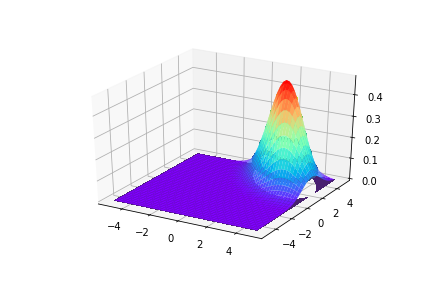
\includegraphics[width=0.32\linewidth]{contour2.png}}
	  %这里是空了一行,能够实现强制将四张图分成两行两列显示,而不是放不下图了再换行,使用\\也行。
	  \\
	\subfigure[$\mu = \begin{bmatrix}1.2 ,& 0.2\end{bmatrix} \sigma= \begin{bmatrix}2 & 0 \\0 & 4 \end{bmatrix} $]{
		\label{level.sub.3}
		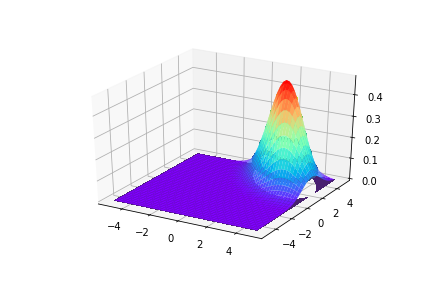
\includegraphics[width=0.32\linewidth]{contour3.png}}
	\quad
	\subfigure[$\mu = \begin{bmatrix}2.4 ,& 3.2\end{bmatrix} \sigma= \begin{bmatrix}2 & 0 \\0 & 2 \end{bmatrix} $]{
		\label{level.sub.4}
		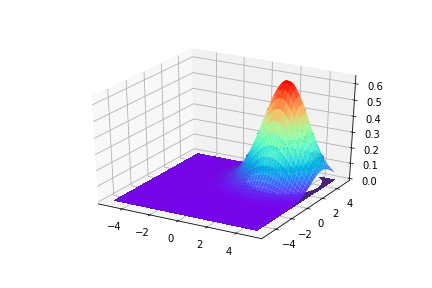
\includegraphics[width=0.32\linewidth]{contour4.png}}
	\caption{3-dimension contours of Bi-variate Gaussian distribution}
	\label{3D contours of Bi-variate Gaussian Distribution}
\end{figure}

\subsection{Distribution of Projections}

Matrix decomposition is the factorization of a matrix into a product of matrices. The LU decomposition and Cholesky decomposition are the most frequently used one. In cholesky decomposition, the matrix A is decomposed into a product of a unique lower triangular matrix L and its transpose: $A=LL^{T}$. In our case, the original data is generated by the product of a uniform random data matrix(matrix X)  and the transpose of the cholesky matrix(matrix A) of the covariance matrix C: $Y=XA^{T}$. Then matrix X and A are plot in Figure 6 to show the change of the dimension.

\begin{wrapfigure}{r}{0.7\textwidth}
\centering 
\vspace{-5mm}
\hspace{20mm}
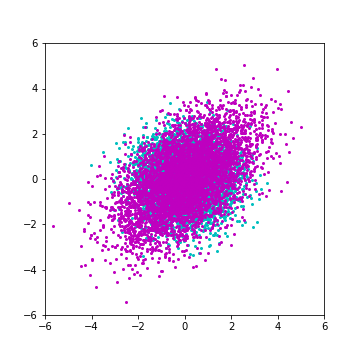
\includegraphics[width=0.7\linewidth]{originalData.png} 
\caption{\footnotesize  The scatter plot of X and Y}
\centering
\end{wrapfigure}

Projection is a technique used to reduce the dimension of a set of points. In this section, the data is projected onto a vector $u=\begin{bmatrix}\sin  \theta & \cos\theta  \end{bmatrix}$, where $\theta$ is a parameter that varies from 0 to $2\pi$. With the change of $\theta$, the data can be projected onto any vector in the area. And, therefore, the variance of the projected data varies with $\theta$. By calculating all the variances of possible projections, we plot a graph(Figure 7) to show how the variance changes as theta varies.

The calculated maxima and minama of the variance are approximately 3.08 and 0.98. And the corresponding angle of projection when variance reaches maxima and minima are 44.08 degress and 315.91 degrees respectively.

Eigen decomposition is the decomposition of a matrix into matrices composed of its eigenvectors and eigenvalues. We can compute the eigenvalues of the covariance matrix C: 
\begin{equation}
    \centering
     \lambda_1 = 3, \lambda_2 = 1
    \centering
\end{equation}
And the corresponding eigenvectors are:
\begin{equation}
    \centering
     u_1=\begin{bmatrix}0.70710678 ,& 0.70710678 \end{bmatrix},
     u_2=\begin{bmatrix}-0.70710678 ,& 0.70710678 \end{bmatrix}
    \centering
\end{equation}
The angle of the eigenvector corresponding to the larger eigenvalue is 45 degrees, which is very close to 44.08, and the angle of projection when variance reaches maxima. And, inversely, the angle of the eigenvector corresponding to the smaller eigenvalue is -45 degrees, which is close to approximately equal to 315.91 degrees. In addition, the larger eigenvalue 3 is close to the maxima of variance, and the smaller eigenvalue 1 is close to the minima of variance. 

Say $\mu$ is the mean of projected data, $e_j$ is the $j^{th}$ element of the eigenvector e. The variance of projected data($x^Te$):
\begin{equation}
\begin{aligned}
      \frac{1}{n}\sum_{n=1}^n\big(\sum_{j=1}^d x_{ij}e_j-\mu\big)^2 =  \frac{1}{n}\sum_{n=1}^n\big(\sum_{j=1}^d x_{ij}e_j\big)^2\\
      = \frac{1}{n}\sum_{n=1}^n\big(\sum_{j=1}^d x_{ij}e_j\big)\big(\sum_{a=1}^d x_{ia}e_a\big)\\
      = \sum_{j=1}^d  \sum_{a=1}^d  \big( \frac{1}{n} \sum_{i=1}^n x_{ia}x_{ij}\big)e_je_a\\
      =\sum_{a=1}^d \big( \sum_{j=1}^dcov(a,j)e_j\big)e_a \\
      =\sum_{a=1}^d (\lambda e_a)e_a = \lambda \parallel e \parallel ^2 = \lambda
\end{aligned}
\end{equation}

where $\mu=\frac{1}{n}\sum_{i=1}^{n} \big( \sum_{ij}^d x_{ij}e_j \big) =  \sum_{j=1}^d  \big( \frac{1}{n} \sum_{i=1}^d x_{ij}\big)e_j =0 $. Then we come to the conclusion, when the eigenvectors are unit vectors, the corresponding eigenvalues are the maximal variance of the projected data. Also, the maxima and minima of the variance always exist in the direction of projection where the eigenvectors are.

We use the Cholesky matrix to create correlations among random variables. For example, suppose that the two columns in matrix X are independent standard normal variables. The matrix A can be used to create new variables Y such that the covariance of the two columns in Y equals C. Then Y has a distribution:$Y \sim N \big(m,C\big) =N\big(0,C\big)$. Then, provided with a unit vector $u= \begin{bmatrix}\sin\theta & \cos\theta \end{bmatrix} $, we make product of them: $Yp = Yu$.

The variance of Yp can be computed as:
\begin{equation}
\begin{aligned}
      u^TCu =  \begin{bmatrix}\sin\theta ,& \cos\theta \end{bmatrix} \begin{bmatrix}2 & 1 \\ 1 & 2 \end{bmatrix} \begin{bmatrix}\sin\theta \\ \cos\theta \end{bmatrix} \\
      = 2 + \sin{2\theta}
\end{aligned}
\end{equation}

The shape of the graph have looked sinusoidal, with a period equal to $\pi$.


\begin{wrapfigure}{r}{0.7\textwidth}
\centering 
\vspace{-5mm}
\hspace{20mm}
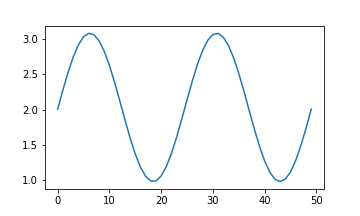
\includegraphics[width=0.7\linewidth]{varianceOfTheProjectedData.png} 
\caption{\footnotesize  Variance of the projected data}
\centering
\end{wrapfigure}
\end{document}